%fix option clash
\PassOptionsToPackage{dvipsnames,usenames}{xcolor}
%https://nuanceabounds.org/fix-latex-package-option-clash-error-passoptionstopackage/

\documentclass[titlepage]{article} 
\usepackage{./style/ferinPackages}

% TITLE %%%%%%%%%%%%%%%%%%%%%%%%%%%%%%%%%%%%%%%%%%%%%%%%%%%%%%%%%%
\title{
%\normalfont \normalsize 
\large APPM 2360 Spring 2022 \\
[10pt] 
\rule{\linewidth}{2pt}  \\[10pt]
\huge Project 2 \\
\LARGE Analysis of the Mariana Trench Utilizing Incomplete Singular Value Decomposition\\
\rule{\linewidth}{2pt}  \\[10pt]
\author{Ferin Von Reich, Ben Scheck, Aaron Groudan}
\date{April  5, 2022}
}

%COMMANDS BEFORE BEGIN %%%%%%%%%%%%%%%%%%%%%%%%%%%%%%%%%%%%%%%%%%%%%%%%%
\doublespacing

%BEGIN DOCUMENT %%%%%%%%%%%%%%%%%%%%%%%%%%%%%%%%%%%%%%%%%%%%%%%%%%%%%%%%%%%%%%%%%%%%%%%%
\begin{document}

%LANGUAGE SETUP TODO: PYTHON %%%%%%%%%%%%%%%%%%%%%%%%%%%%%%%%%%%%%%%%%%%%%%%%%%%%%%%%%%%
\lstset{language=Matlab,%
    %basicstyle=\color{red},
    breaklines=true,%
    morekeywords={matlab2tikz},
    keywordstyle=\color{blue},%
    morekeywords=[2]{1}, keywordstyle=[2]{\color{black}},
    identifierstyle=\color{black},%
    stringstyle=\color{mylilas},
    commentstyle=\color{mygreen},%
    showstringspaces=false,%without this there will be a symbol in the places where there is a space
    numbers=left,%
    numberstyle={\tiny \color{black}},% size of the numbers
    numbersep=9pt, % this defines how far the numbers are from the text
    emph=[1]{for,end,break},emphstyle=[1]\color{red}, %some words to emphasise
    %emph=[2]{word1,word2}, emphstyle=[2]{style},    
}

%Format and  intial stuff %%%%%%%%%%%%%%%%%%%%%%%%%%%%%%%%%%%%%%%%%%%%%%%%%%%%%%%%%%%%%%%%%%%%%%%%%%%%%%%%
\maketitle
\tableofcontents
\newpage


%DOCUMENT START %%%%%%%%%%%%%%%%%%%%%%%%%%%%%%%%%%%%%%%%%%%%%%%%%%%%%%%%%%%%%%%%%%%%%%%%%%%%
\section{Introduction} \label{sec:intro}
The Mariana Trench, lying in the Pacific Ocean between Japan and Papua New Guinea, is the deepest trench in the world. Because of its steep sides and vast depth, the trench provides a unique environment for scientific study. In this project, we will use bathymetric data provided by the United States National Oceanic and Atmospheric Administration (NOAA) to conduct an investigation of the trench. In addition, because this data is often difficult to work with, containing thousands of values, we will explore a means to reduce the size of the data while simultaneously maintaining the structure of the trench. This will allow for further, more computationally intensive investigation.


%%%%%%%%%%%%%%%%%%%%%%%%%%%%%%%%%%%%%%%%%%%%%%%%%%%%%%%%%%%%%%%%%%%%%%%%%%%%%%
\section{Initial Investigation}  \label{sec:initInvest}
On initial investigation of the data, one finds that the Mariana trench is represented by three matrices. The matrices represent the depth (size $1320 \times 1440$), longitude (size $1320 \times 1$), and latitude (size $1440 \times 1$) of the data recorded. In the future we will refer to the depth matrix as $\matr{A}$. Plots of the data can be seen in \autoref{fig:intialMarianaMesh}
\begin{figure}[H]
    \centering
    \subfloat[\centering 3D Plot of $\mtrA$]
    {{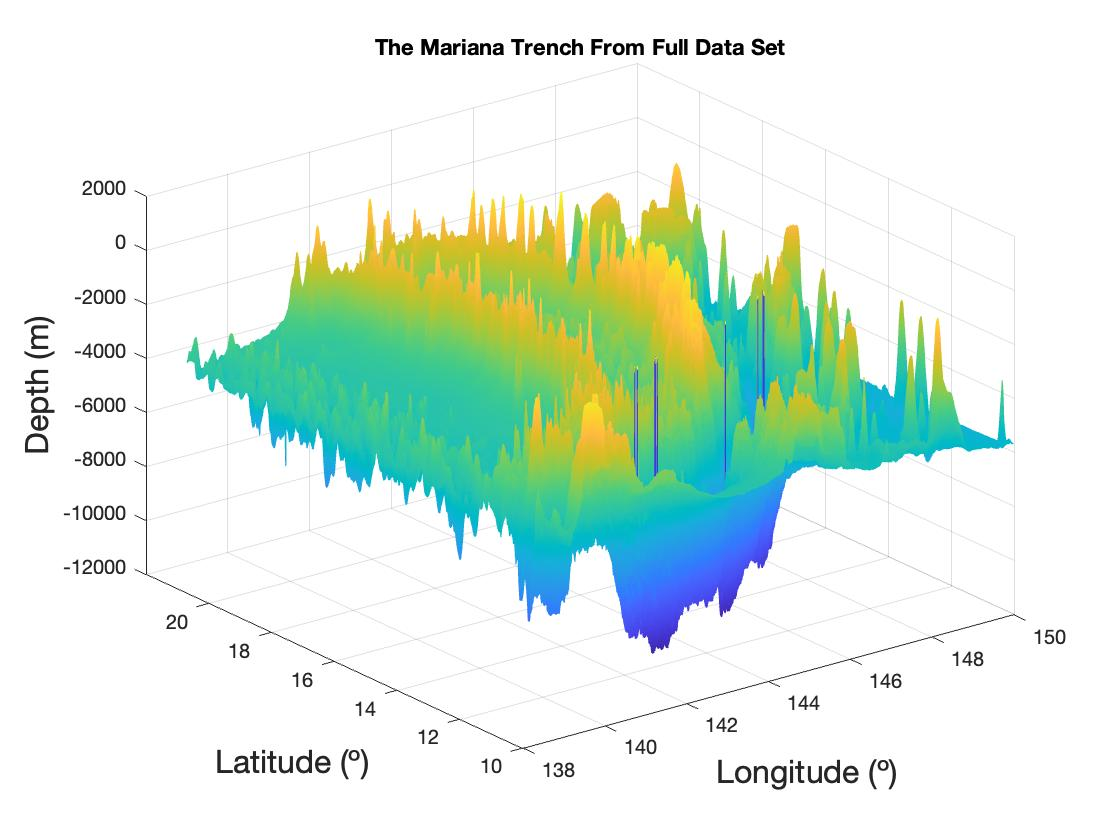
\includegraphics[width=0.45\textwidth]{./imgs/trueDataRendering.jpg}}}%
    \qquad
    \subfloat[\centering 2D Plot of $\mtrA$]
    {{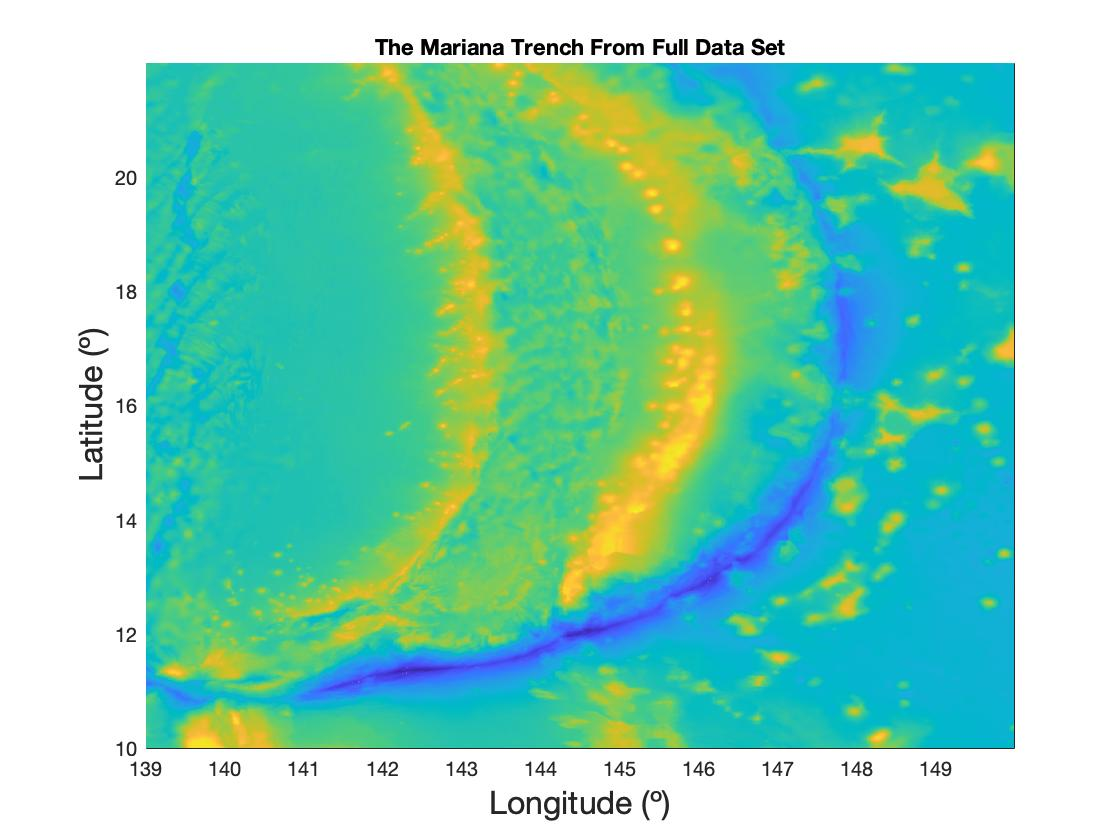
\includegraphics[width=0.45\textwidth]{./imgs/twoDFullDataSet.jpg}}}%
    \caption{Plots of Mariana Trench Depth, $\matr{A}$, in terms of latitude and longitude}%
    \label{fig:intialMarianaMesh}%
\end{figure}
Exploring this data, we find that the deepest point in the trench is $10.93$ km below sea level at a latitude of $11.333\degree$ and a  longitude of $142.2\degree$. See Section \ref{sec:codeWithOutput} for the code used. In addition, nominally defining the ocean floor to have a depth of $6$ kilometers, we can find the average depth of the trench by finding the mean of the values below 6 kilometers in $\matr{A}$. Thus, we find the average depth of the Mariana Trench to be $7.205$ km. See Section \ref{sec:codeWithOutput} for the computation used.

%%%%%%%%%%%%%%%%%%%%%%%%%%%%%%%%%%%%%%%%%%%%%%%%%%%%%%%%%%%%%%%%%%%%%%%%%%%%%%

\section{Singular Value Decomposition}  \label{sec:svd}
At this point, conducting further investigation would be impractical as the size of $\matr{A}$ is too large to quickly compute with. Thus, it is necessary to find a way to reduce the size of the data while preserving the structure of the trench. To simplify the data, we must first understand the concept of Singular Value Decomposition (SVD). 


SVD is a factorization of a matrix that breaks up a matrix into three separate matrices such that $\matr{A} = \matr{U}\matr{\Sigma}\matr{V}^T$, where $\matr{U}$ and $\matr{V}$ are orthogonal matrices and $\matr{\Sigma}$ is a diagonal matrix. A pictorial representation of this can be seen in \autoref{fig:svdA}
\begin{figure}[H]
    \centering
    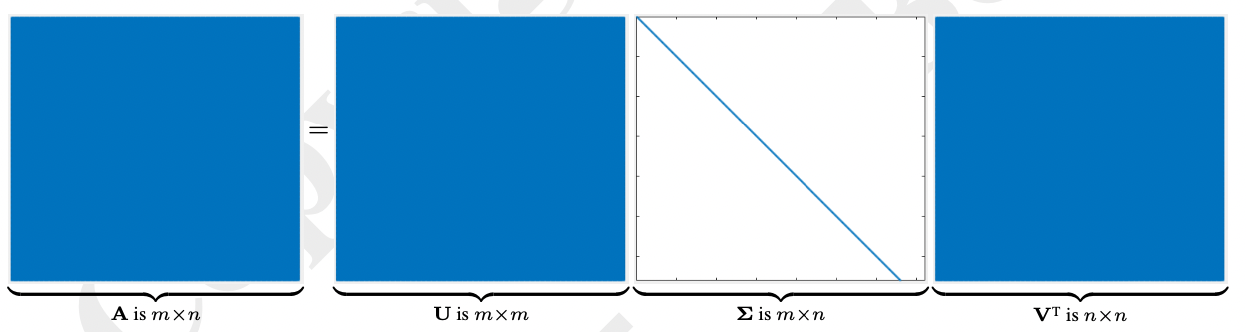
\includegraphics[width=\textwidth]{./imgs/SVD.jpg}
    \caption{SVD Representation of $\mtrA$}
    \label{fig:svdA}
\end{figure}
 As with standard factorization, each of the three matrices tell you information about the parent matrix $\mtrA$. $\mtrSig$  contains the singular values which are the square roots of the eigenvalues of $\matr{A}^T\matr{A}$ and $\mtrV$ represents the associated eigenvectors of those eigenvalues. $\mtrU$ contains the eigenvectors of $\matr{A}\matr{A}^T$. Physically interpreted,  the columns of $\matr{V}$ represent a basis of $\RR^n$ and the columns of $\matr{U}$ represent a basis of $\RR^m$. Written mathematically, this means:
 \begin{align*}
     \mtrA\mvec{x} &= \mtrA( c_1\mvec{V}_1 + c_2\mvec{V}_2 + \dots + c_n\mvec{V}_n)\\
     &= c_1\mtrSig_{11}\mvec{U}_1 +  c_2\mtrSig_{22}\mvec{U}_2 + \dots + c_n\mtrSig_{mm}\mvec{U}_m 
 \end{align*}

%%%%%%%%%%%%%%%%%%%%%%%%%%%%%%%%%%%%%%%%%%%%%%%%%%%%%%%%%%%%%%%%%%%%%%%%%%%%%%

\section{Incomplete Singular Value Decomposition}  \label{sec:isvd}
While SVD is useful for a deeper understanding of the parent matrix, it still does not reduce the number of values needed to represent the parent matrix. In fact, as one can see from \autoref{fig:svdA} the SVD matrices will actually require more values than the parent matrix. However, if we order the singular values and vectors such that $\mtrSig_{11} \ge  \mtrSig_{22} \ge \dots \ge \mtrSig_{mm}$, then for some $k<m$ we can make the approximation:
 \begin{align*}
     \mtrA\mvec{x} &= c_1\mtrSig_{11}\mvec{U}_1 +  c_2\mtrSig_{22}\mvec{U}_2 + \dots + c_n\mtrSig_{mm}\mvec{U}_m \\
     &\approx c_1\mtrSig_{11}\mvec{U}_1 +  c_2\mtrSig_{22}\mvec{U}_2 + \dots + c_n\mtrSig_{kk}\mvec{U}_k \tag{where $k < m$} 
 \end{align*}
This is to say that we are cutting off the action of matrix $\mtrA$ a little early, but, because of the ordering, we are losing as little information as possible. This is called the Incomplete Singular Value Decomposition (ISVD), where we preserve essence of the completed SVD, but it assumes the large  elements of $\mtrSig$ and the corresponding columns in $\mtrU$ and $\mtrV$ matter most, throwing away the columns that are less useful. This will thus allow us to reduce the values need to represent $\mtrA$. This is shown pictorially in \autoref{fig:isvdA}.
\begin{figure}[H]
    \centering
    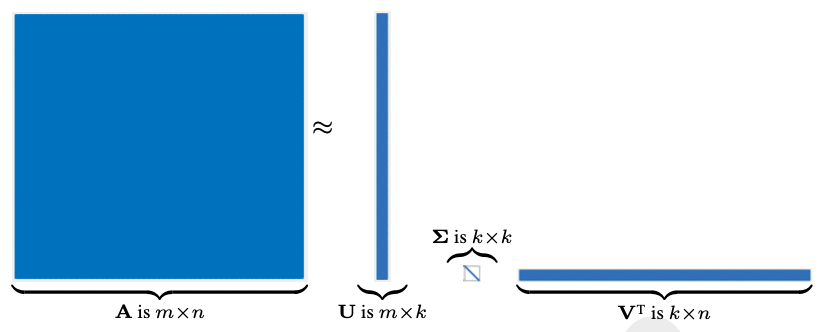
\includegraphics[width=0.6\textwidth]{./imgs/ISVD.jpg}
    \caption{ISVD Representation of $\mtrA$}
    \label{fig:isvdA}
\end{figure}
%%%%%%%%%%%%%%%%%%%%%%%%%%%%%%%%%%%%%%%%%%%%%%%%%%%%%%%%%%%%%%%%%%%%%%%%%%%%%%

\section{Computing the First Eigenvalue and Eigenvector of ATA} \label{sec:firstEigen}
Having described the mathematical foundation for ISVD, we will now explore its programmatic implementation. First, we need a method to find an eigenvalue from a matrix. To find the first eigenvector, and in turn the first eigenvalue of the depth matrix $\mtrA$, we can use the following algorithm:
\begin{center}
\begin{enumerate}
    \item Guess a random unit vector with size corresponding to $\mtrA$ (in the case of the Mariana Trench $1440$).
    \item Multiply $\mtrA^T\mtrA$ by the guess vector and divide the result by its magnitude to define the next unit vector.
    \item Use the newly defined unit vector as the updated guess.
    \item Repeat steps $3$ and $4$ until the vector stops changing, this is the first eigenvector $\mvec{V}_1$.
\end{enumerate}
\end{center}
Defined more mathematically, this algorithm is represented as:
\begin{enumerate}
    \item $\mvec{u}_1 = $  a random unit vector with the correct number of components.
    \item $\mvec{u}_{n+1} := \frac{\mtrA^T\mtrA\mvec{u}_{n}}{\lVert \mtrA^T\mtrA\mvec{u}_{n} \rVert}$
    \item Repeat using $\mvec{u}_{n+1}$ as the guess until $\lVert \mvec{u}_{n+1} -  \mvec{u}_{n} \rVert < \text{acceptable precision}$
\end{enumerate}
Note that $\lVert \mvec{u} \rVert$ is the magnitude of the vector $\mvec{u}$ that has $N$ components. Thus, it is defined as:
\begin{align*}
    \lVert\mvec{u}\rVert=\sqrt{\sum \:\:_{i=1}^Nu_i^2}
\end{align*}

Further exploration of why this algorithm works is necessary in a future project. However, a hypothesis as to why this algorithm works could be that we know that the vector ${\mvec{u}_{n}}$ can be expressed using the basis of the eigenvectors from $\mtrA^T\mtrA$, meaning that:
\begin{align*}
    \mtrA^T\mtrA{\mvec{u}_{n}} &= {\mvec{u}_{n}}(\lambda_1\mvec{V_1}\mvec{V_1}^T+\lambda_2\mvec{V_2}\mvec{V_2}^T+...+\lambda_n\mvec{V_n}\mvec{V_n}^T) \\
    &= {\mvec{u}_{n}\lambda_1}(\mvec{V_1}\mvec{V_1}^T+\frac{\lambda_2}{\lambda_1}\mvec{V_2}\mvec{V_2}^T+...+\frac{\lambda_n}{\lambda_1}\mvec{V_n}\mvec{V_n}^T)  \tag{factoring out $\lambda_1$}
\end{align*}
Note that since we are computing the largest eigenvalue, we are assuming that $\lambda_1 >> \lambda_{2...n}$. Then, we normalize the vector so that it has magnitude 1, and perform the multiplication. We repeat this over, and over, lets say we repeat it $g$ times. Then, we can say that:
\begin{align*}
    \mtrA^T\mtrA{\mvec{u}_{n}} 
    &= {\mvec{u}_{n}\lambda_1^g}(\mvec{V_1}\mvec{V_1}^T+(\frac{\lambda_2}{\lambda_1})^g\mvec{V_2}\mvec{V_2}^T+...+(\frac{\lambda_n}{\lambda_1})^g\mvec{V_n}\mvec{V_n}^T) \\  
    &= {\mvec{u}_{n}\lambda_1^g}\mvec{V_1}\mvec{V_1}^T \tag{assuming that $\lambda_1 >> $ all other eigenvalues}\\
    &= {\lambda_1^g}\mvec{V_1}\mvec{V_1}^T  \tag{$\mvec{u}$ is a unit vector, so it is negligible}\\
    &= {\lambda_1^g}
\end{align*}
In other words, as we continue to perform the multiplication and normalization, the eigenvalue ratios go closer and closer to 0, since we are under the assumption that the first eigenvalue is the largest. Then, after enough multiplications, we can estimate those ratios to be zero, leaving a term that can be manipulated to provide the eigenvalue.

Having thus described the algorithm for finding the largest eigenvalue, we can now implement it on our data. Using this algorithm in Matlab (See Section \ref{sec:codeWithOutput}), we find that for the depth matrix $\mtrA$, the first eigenvector, denoted $\mvec{V}_1$, has an eigenvalue of $3.8802*10^{13}$. In addition, we can inspect the components by looking at the plot of $\mvec{V}_1$ as show in \autoref{fig:firstEVect}.
\begin{figure}[H]
    \centering
    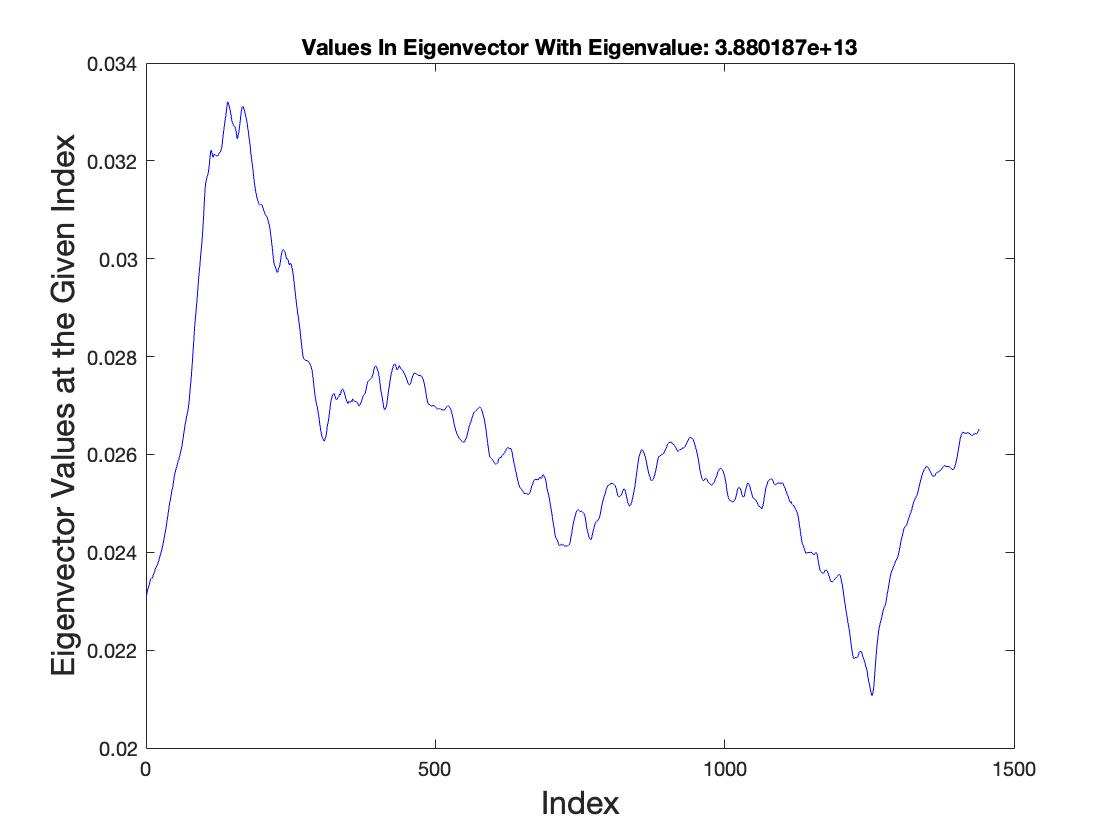
\includegraphics[width=0.6\textwidth]{./imgs/eVect1.jpg}
    \caption{Plot of the Components of $\mvec{V}_1$}
    \label{fig:firstEVect}
\end{figure}
%%%%%%%%%%%%%%%%%%%%%%%%%%%%%%%%%%%%%%%%%%%%%%%%%%%%%%%%%%%%%%%%%%%%%%%%%%%%%%
\section{Computing the 50 Largest Eigenvalues of ATA} \label{sec:50eigen}
Having now found a way to compute an eigenvalue given a matrix, we need a way to calculate the $i$ largest eigenvalues and and associated eigenvectors in order to perform ISVD. To do this, we can use the fact that every eigenvector in a symmetric matrix, for example $\mtrA^T\mtrA$, must be orthogonal to every other eigenvector. Thus, we can modify our algorithm for finding an eigenvalue from Section \ref{sec:firstEigen}
to ensure that the vector that we are currently constructing is orthogonal to every eigenvector we
have already constructed. In other words, if we are in the midst of computing eigenvector $\mvec{V}_i \approx \mvec{u}_n$ then we want to ensure that $\mvec{u}_{n+1}^{T}\mvec{V}_1=\mvec{u}_{n+1}^{T}\mvec{V}_2=\mvec{u}_{n+1}^{T}\mvec{V}_{i-1}=0$.

To do this, we can utilize  \textit{Gram-Schmidt Orthogonalization}. Specifically, from
a next guess vector $\mvec{u}_{n+1}^{*} =\ \mtrA^T\mtrA\mvec{u}_{n}$ having previously computed 
$r$ eigenvectors $\mvec{V}_1 \dots \mvec{V}_r$, we can "orthogonalize" the vector by computing:
\begin{equation*}
    \mvec{u}_{n+1} = \mvec{u}_{n+1}^{*}-\sum _{j=1}^{r-1}\left(\mvec{u}_{n+1}^{* T\:}\mvec{V_j}\right)\mvec{V_j}
\end{equation*}

Relying on these ideas, we can now alter our algorithm from Section \ref{sec:firstEigen} to compute the $i=50$ largest eigenvalues and associated eigenvectors of $\mtrA^T\mtrA$. This creates the following algorithm to assign the eigenvectors to the
matrix $\mtrV$:
\begin{enumerate}
    \item  Initialize $\mvec{V}_1$ to $\mvec{V}_{50}$ as a matrix of zeroes (in this case of the Mariana Trench, this matrix will have size $1440 \times 50$))
    \item for $i=1$ to $50$
    \begin{enumerate}
    \item $\mvec{u}_1 = $  a random unit vector with the correct number of components.
    \item $\mvec{u}_{n+1}^{*} :=\ \mtrA^T\mtrA\mvec{u}_{n} $
    \item $\mvec{u}_{n+1} := \mvec{u}_{n+1}^{*}-\sum _{j=1}^{i-1}\left(\mvec{u}_{n+1}^{* T\:}\mvec{V_j}\right)\mvec{V_j}$
    \item $\mvec{u}_{n+1} := \frac{\mvec{u}_{n+1}}{\lVert\mvec{u}_{n+1}\rVert}$
    \item Repeat b-d until $\lVert \mvec{u}_{n+1} -  \mvec{u}_{n} \rVert < \text{acceptable precision}$
    \item Store the final $\mvec{u}_{n+1}$ as $\mvec{V}_i$
    \end{enumerate}
\end{enumerate}
Converting this algorithm into Matlab, we are now able to compute the $50$ largest eigenvalues, via their eigenvectors, of $\mtrA^T\mtrA$. Again, $\mtrA$ represents the depth data for the Mariana Trench. See Section \ref{sec:codeWithOutput} for the code used for the calculation. Having calculated these eigenvalues, with the corresponding eigenvectors stored as $\mtrV$, we can now create a semilog plot of them, as shown in \autoref{fig:50EVect}.
\begin{figure}[H]
    \centering
    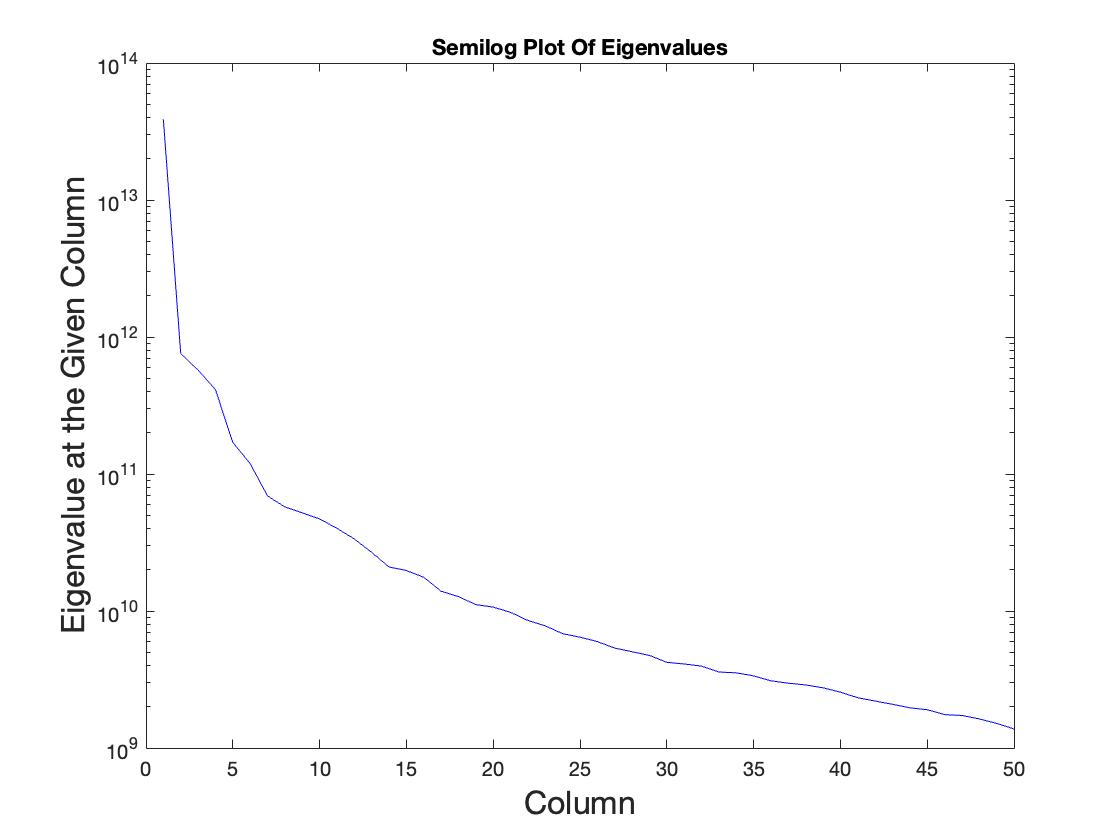
\includegraphics[width=0.6\textwidth]{./imgs/EigenvaluesFor50.jpg}
    \caption{Semilog Plot of the 50 Largest Eigenvalues of $\mtrA^T\mtrA$ \\ Note: Eigenvalues from Columns of $\mtrV$}
    \label{fig:50EVect}
\end{figure}

%%%%%%%%%%%%%%%%%%%%%%%%%%%%%%%%%%%%%%%%%%%%%%%%%%%%%%%%%%%%%%%%%%%%%%%%%%%%%%
\section{Conclusion} \label{sec:conc}

In this project, we analyzed a model of the Mariana Trench, with data from the NOAA. We first did a basic investigation wherein we graphed a representation of the depth data (matrix $\mtrA$), found the deepest point in the trench, and found the average depth of the trench. Then, we described the process of Singular Value Decomposition, and how Incomplete Singular Value Decomposition could be used to reduce the memory needed to represent a data set. Thereafter, we described a method to find the largest eigenvalue in a matrix, and used that algorithm to find the largest eigenvalue in $\mtrA^T\mtrA$. Next, we modified that method to find that largest $i$ eigenvalues of a matrix (where $i$ is an arbitrary constant) and used the resulting algorithm to find the largest $50$ eigenvalues of $\mtrA^T\mtrA$. Afterwards, we explained how to use these eigenvalues to construct the ISVD of a matrix, and used this method to generate numerous ISVD representations of the Mariana Trench, using different numbers of eigenvalues. Then, we quantified how much fewer values are needed to represent the depth of the Mariana Trench using ISVD. Penultimately, we demonstrated that using $50$ eigenvalues, the ISVD representation of the Mariana Trench is very close to the real data, meaning further analysis can be conducted on the ISVD representation without significantly affecting the quality of results. Finally, we showed how the fidelity of the ISVD representation increases as the number of eigenvalues used increases, in turn causing the total number of values used to increase. 


%%%%%%%%%%%%%%%%%%%%%%%%%%%%%%%%%%%%%%%%%%%%%%%%%%%%%%%%%%%%%%%%%%%%%%%%%%%%%%
\newpage
\section{Appendix}\label{sec:append}
\subsection{2D Plots of ISVD with Varying Number of Eigenvalue} \label{sec:isvdCompare2d}
\begin{figure}[H]
    \centering
    \subfloat[\centering Using $1$ Eigenvalue]
    {{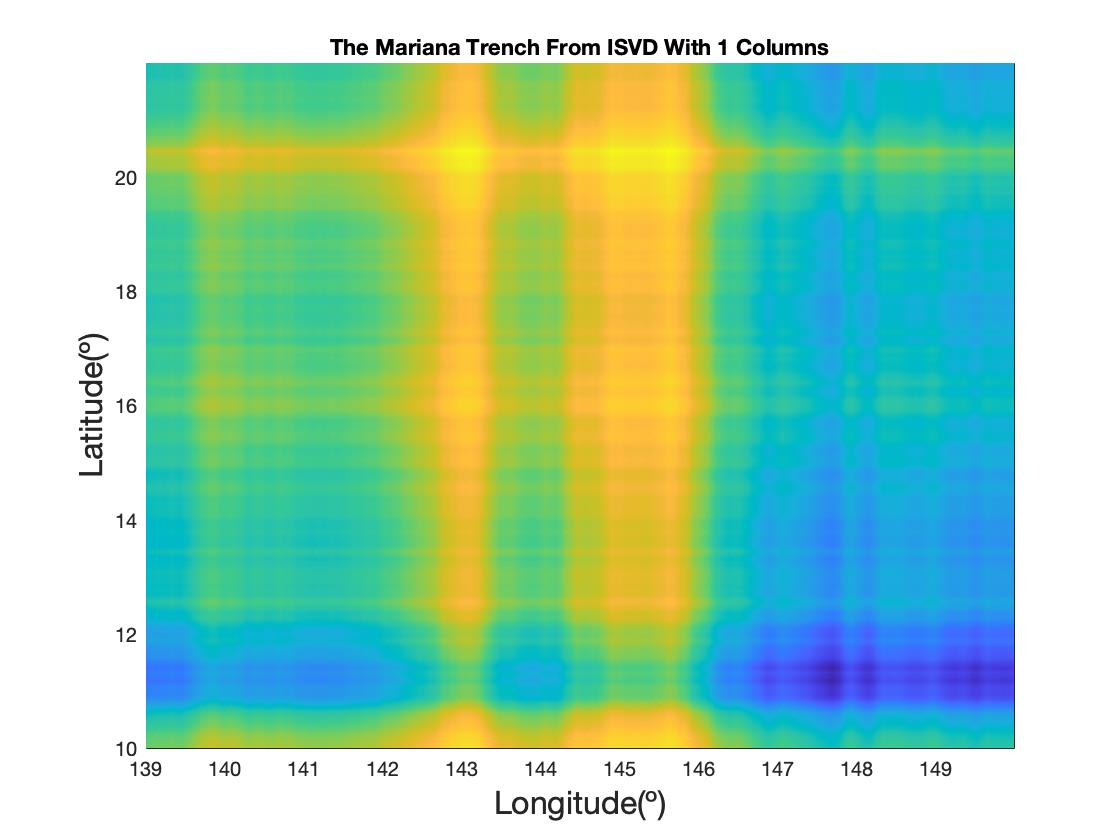
\includegraphics[width=0.45\textwidth]{./imgs/twoD1Col.jpg}}}%
    \qquad
    \subfloat[\centering Using $10$ Eigenvalues]
    {{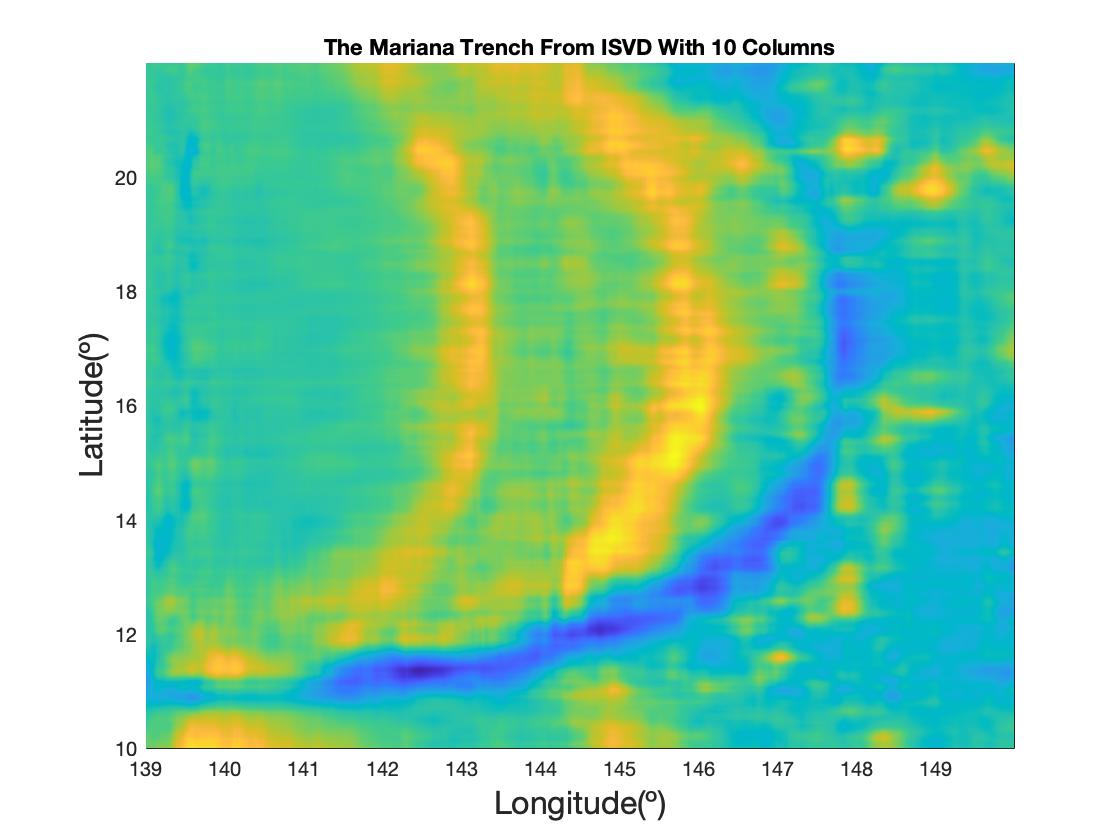
\includegraphics[width=0.45\textwidth]{./imgs/twoD10Col.jpg}}} \\
    \subfloat[\centering Using $100$ Eigenvalues]
    {{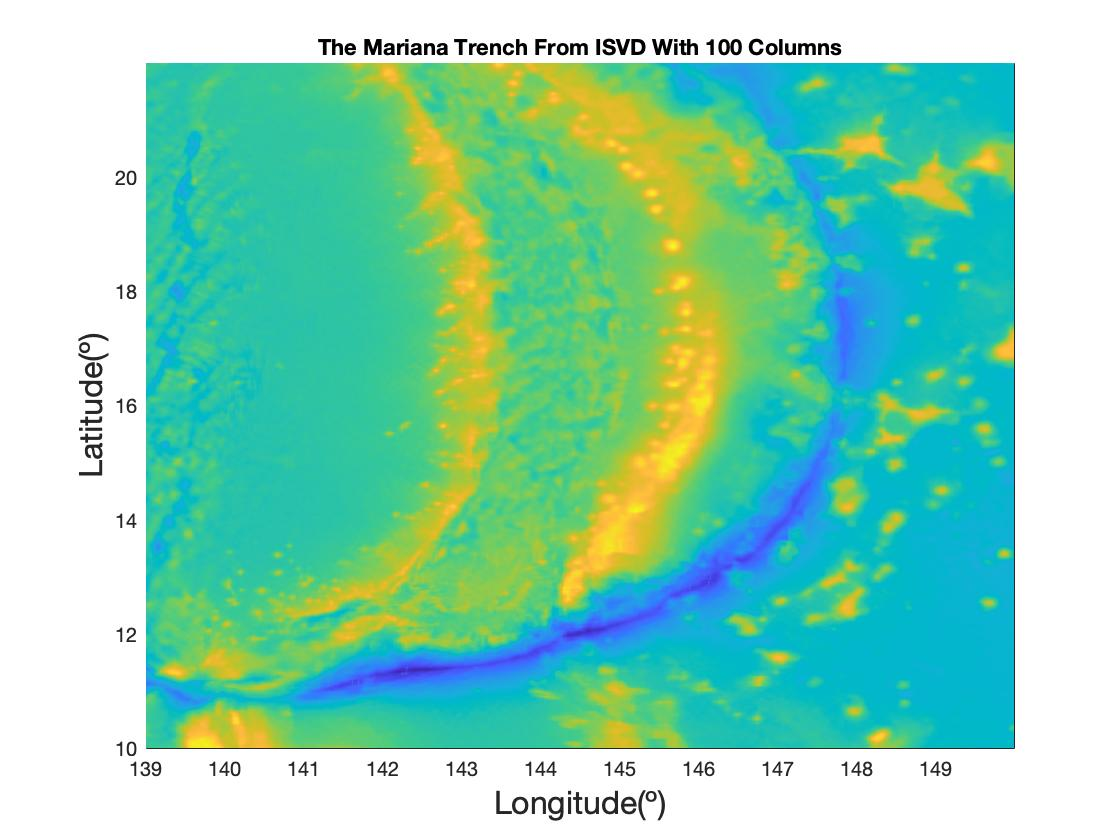
\includegraphics[width=0.45\textwidth]{./imgs/2D100Col.jpg}}}%
    \qquad
    \subfloat[\centering Using $500$ Eigenvalues]
    {{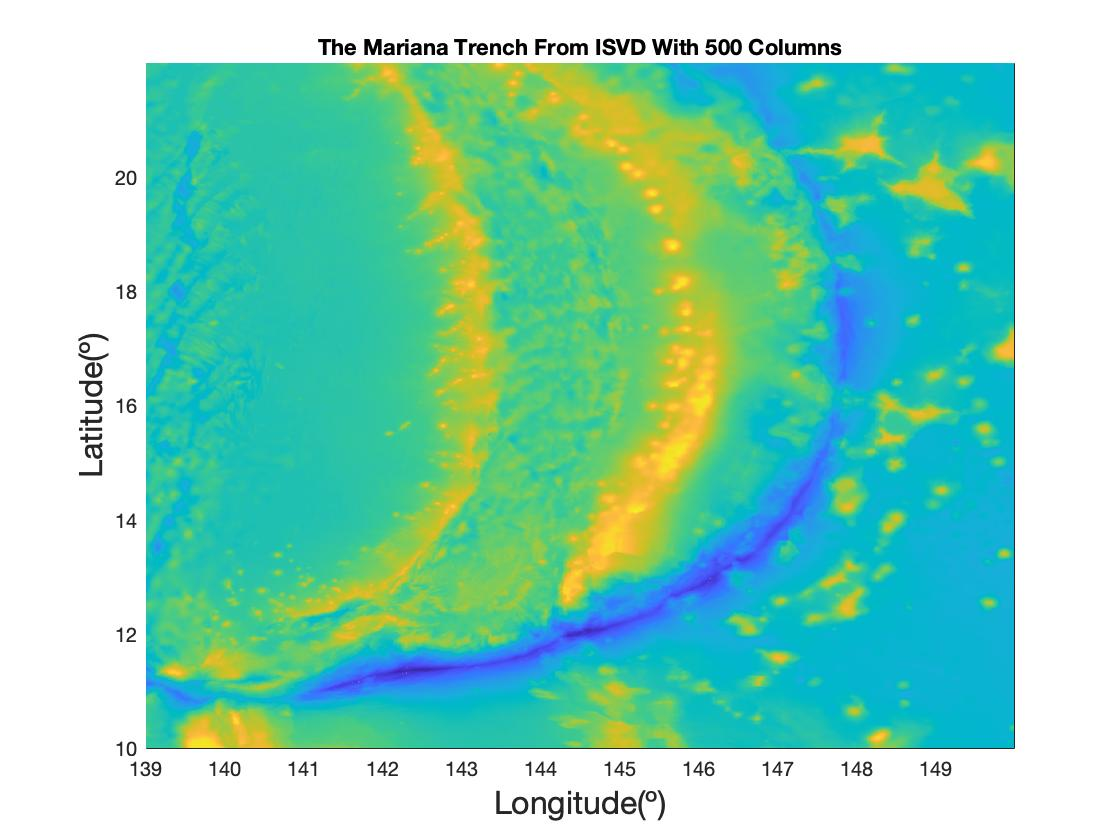
\includegraphics[width=0.45\textwidth]{./imgs/2D500C0l.jpg}}}%
    \caption{2D Plots of ISVDs Using Different Numbers of Eigenvalues for Comparison}%
    \label{fig:comparison2D}%
\end{figure}
\subsection{Code With Output for Reference} \label{sec:codeWithOutput}
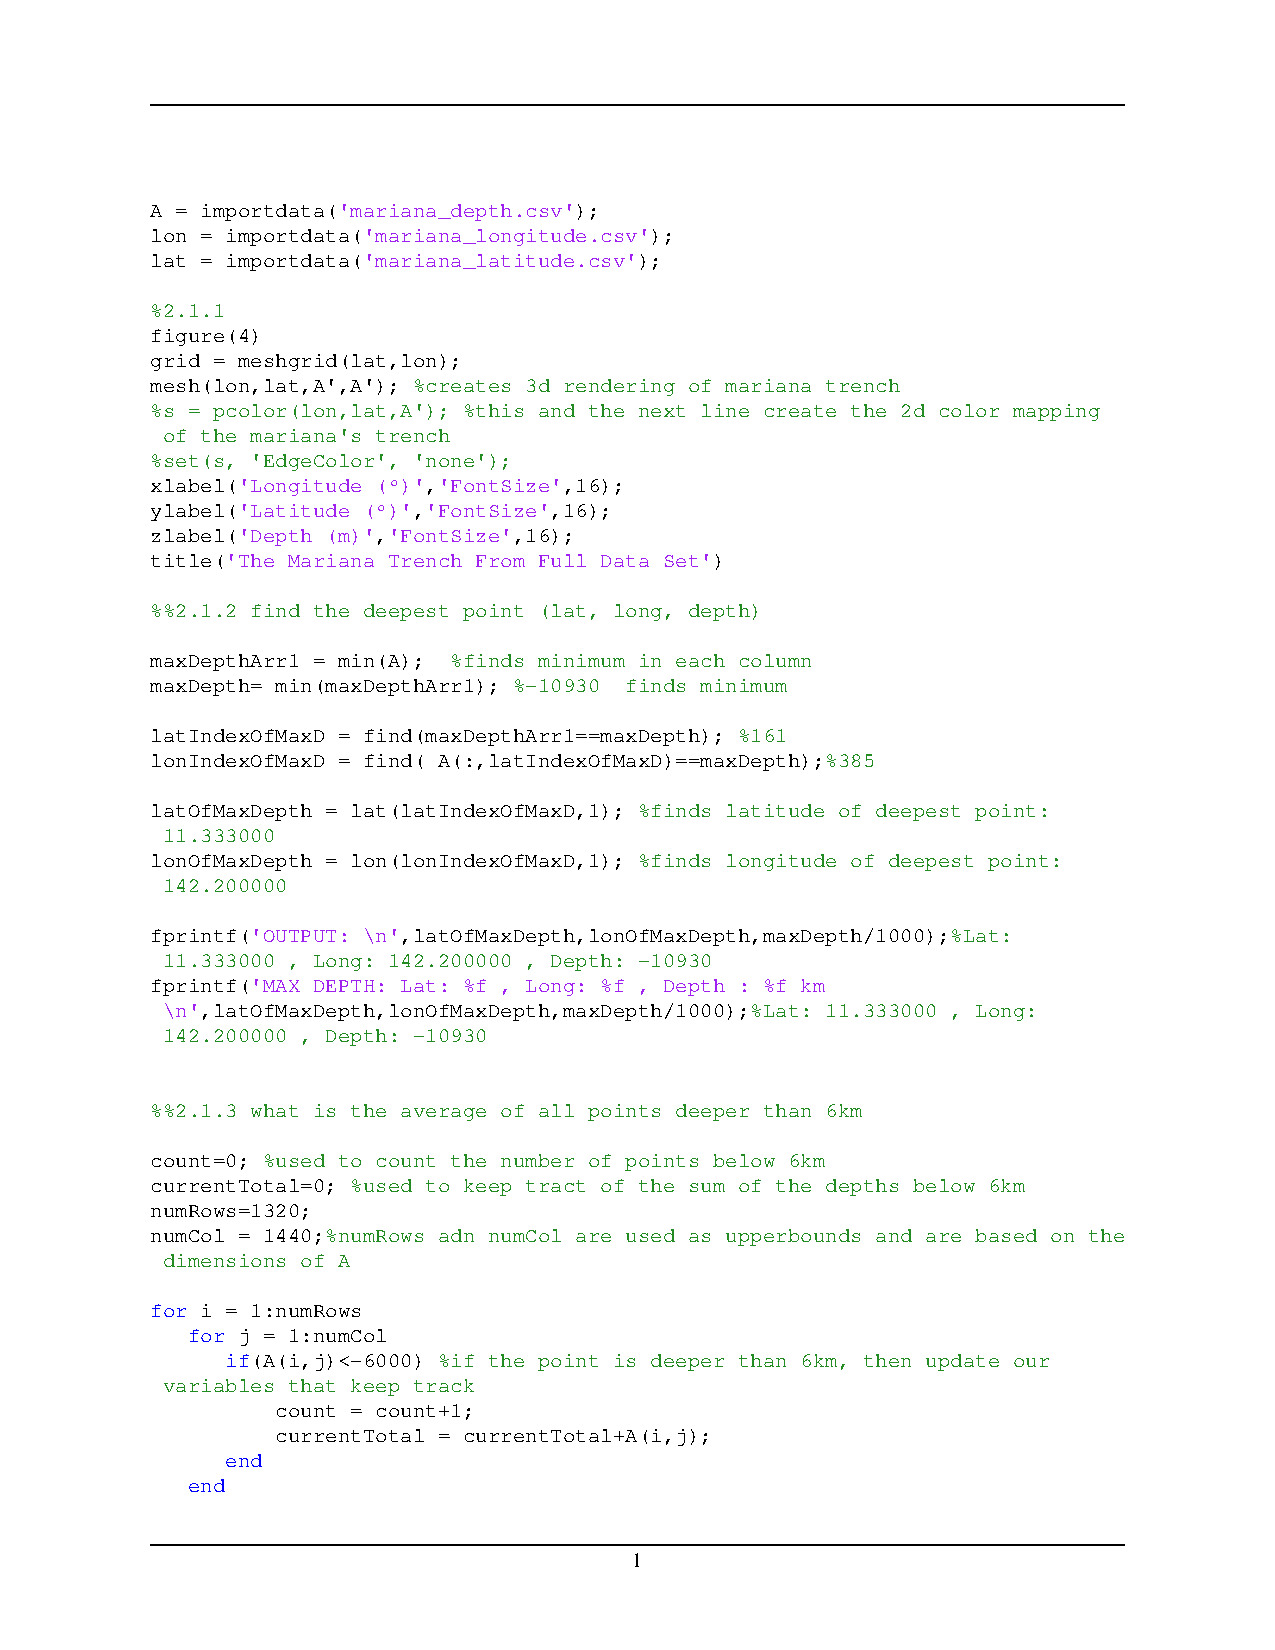
\includepdf[pages=-]{./referenceCode/Part21.pdf}
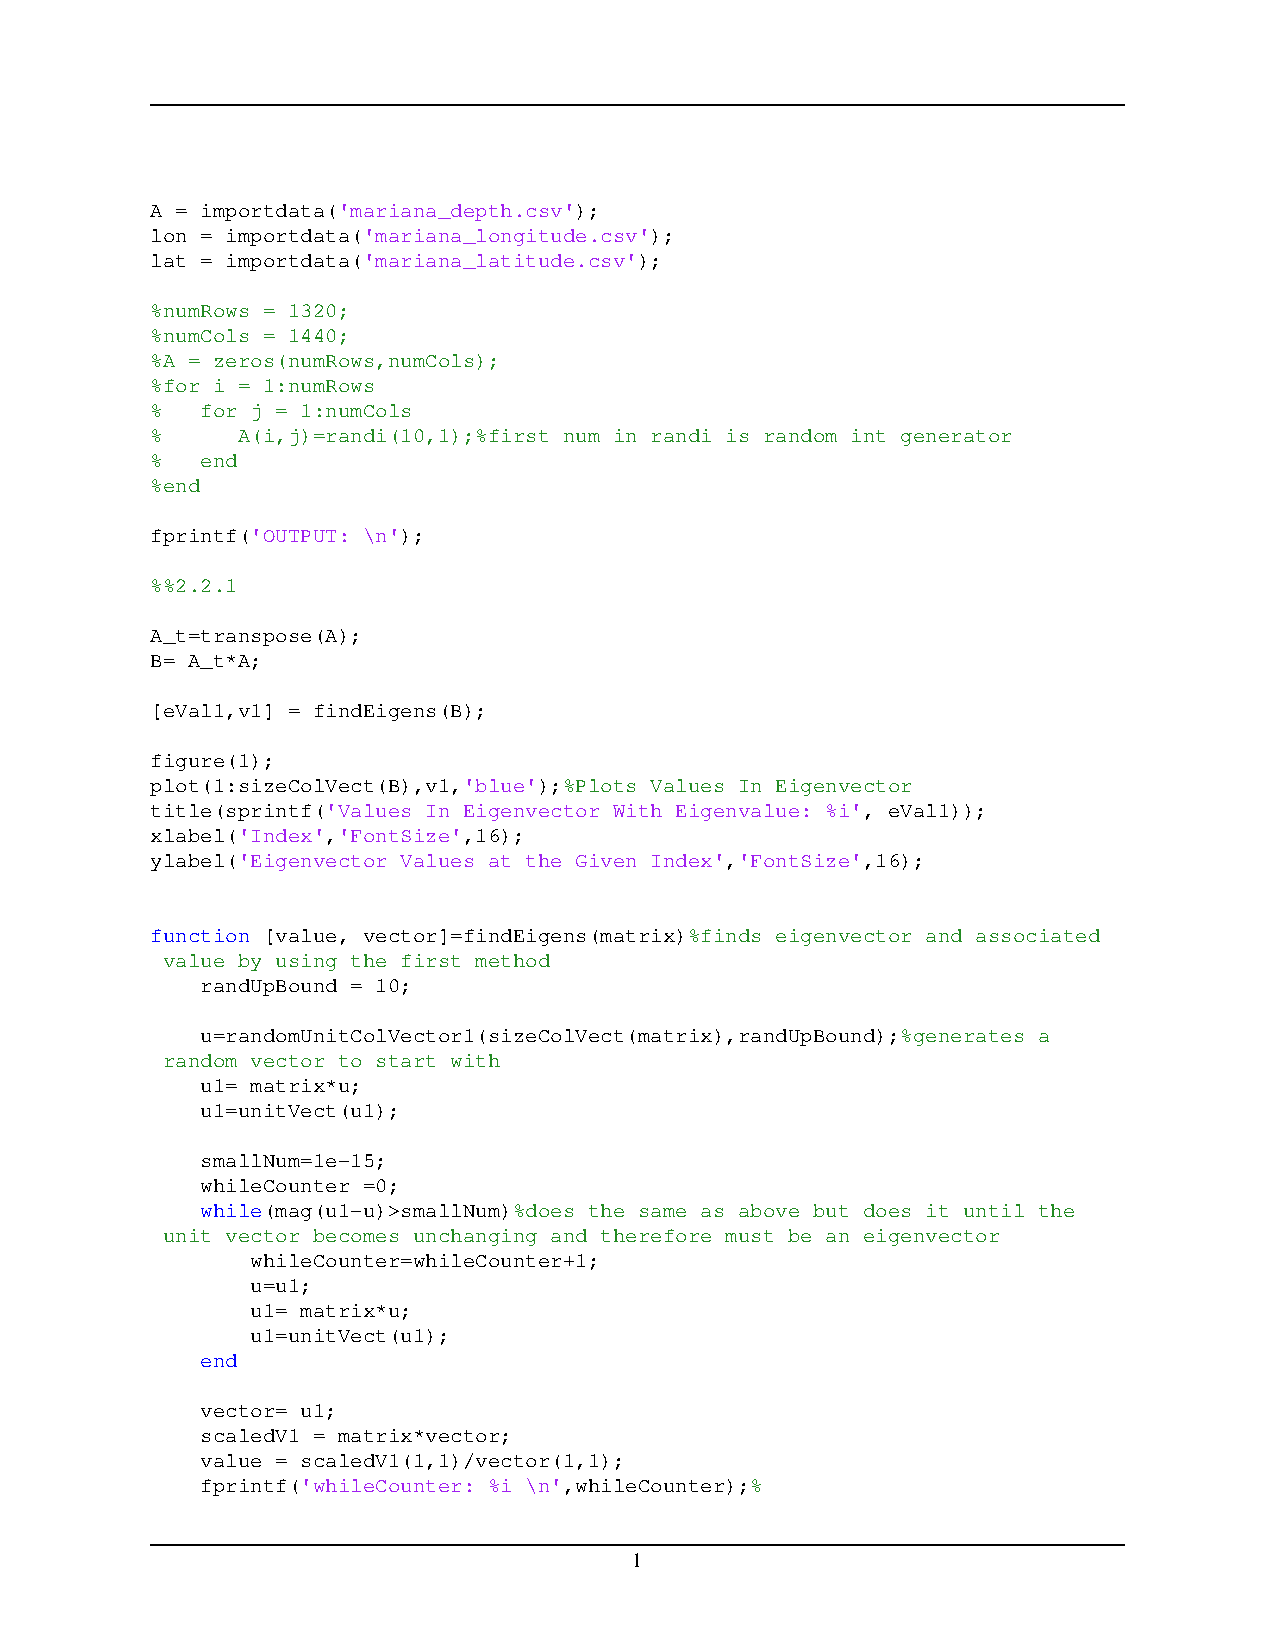
\includepdf[pages=-]{./referenceCode/Part221.pdf}
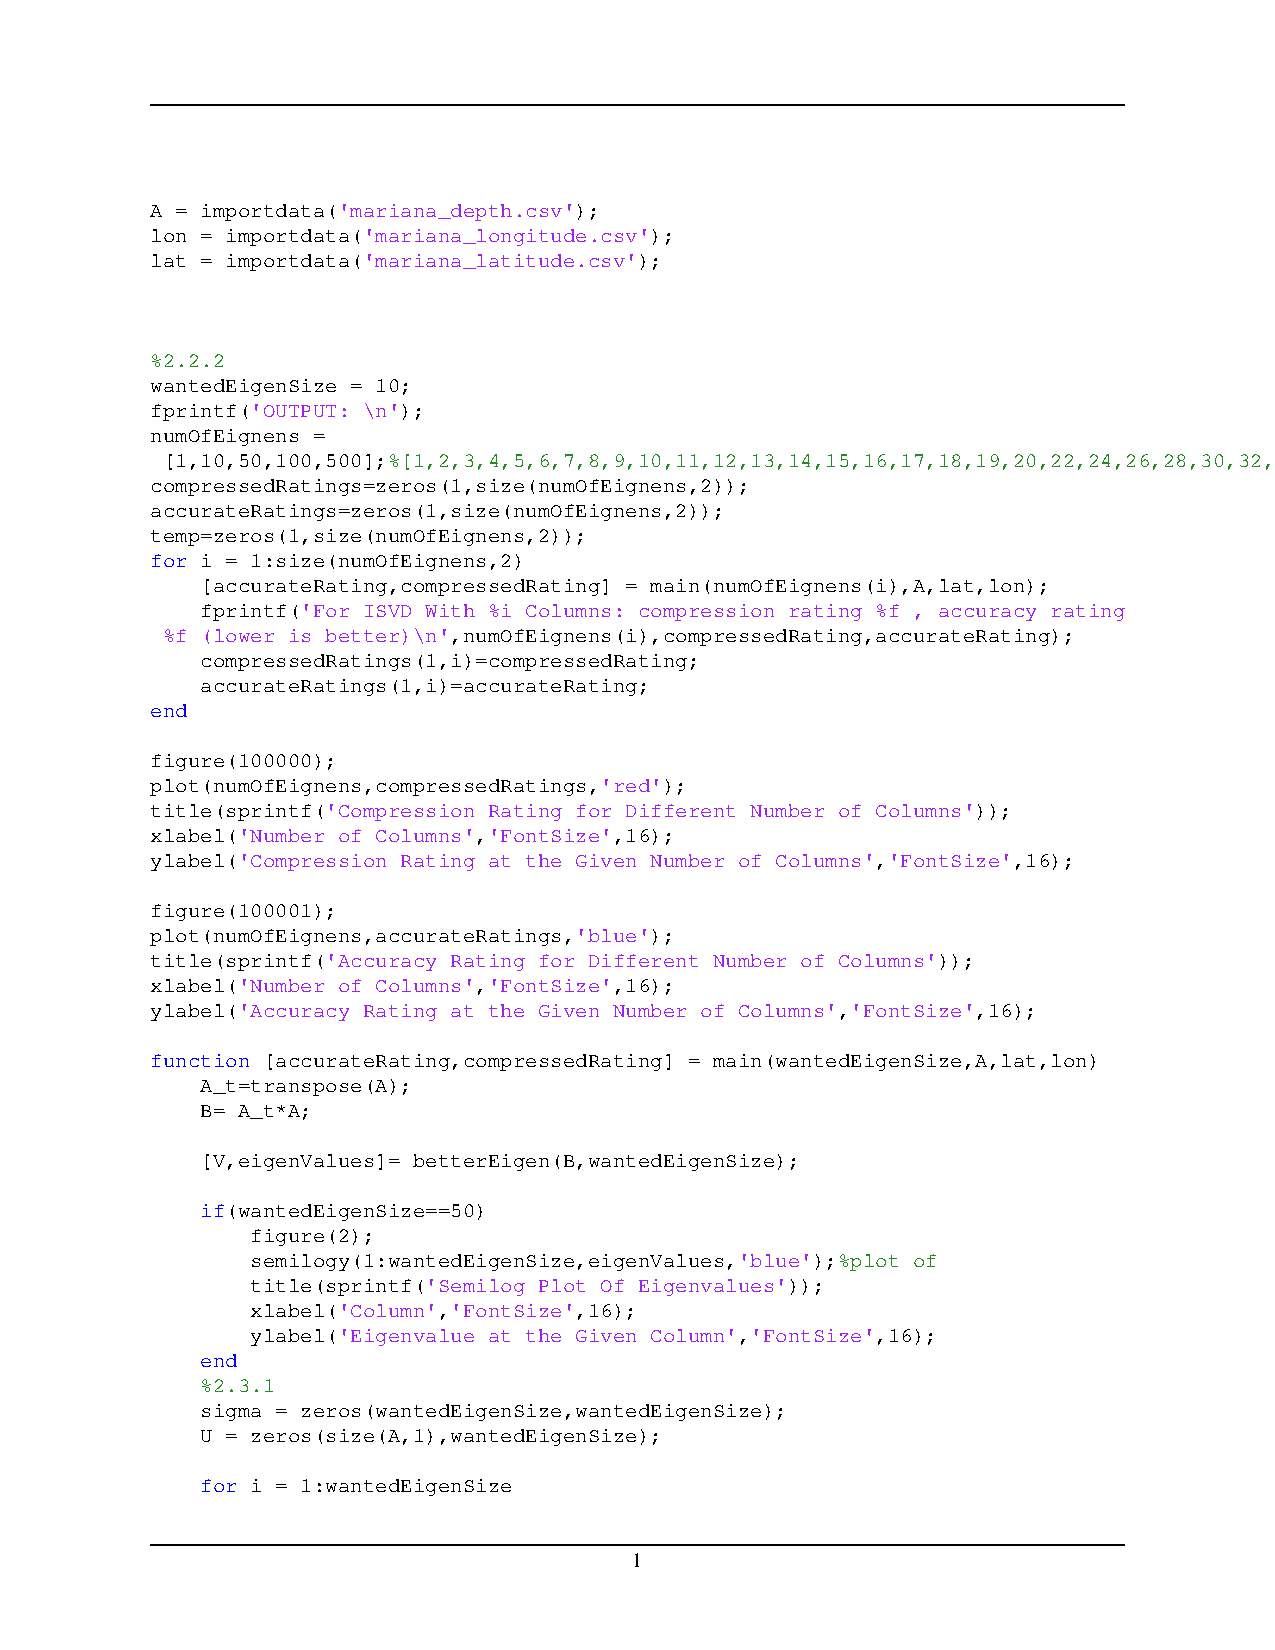
\includepdf[pages=-]{./referenceCode/Part2223D.pdf}
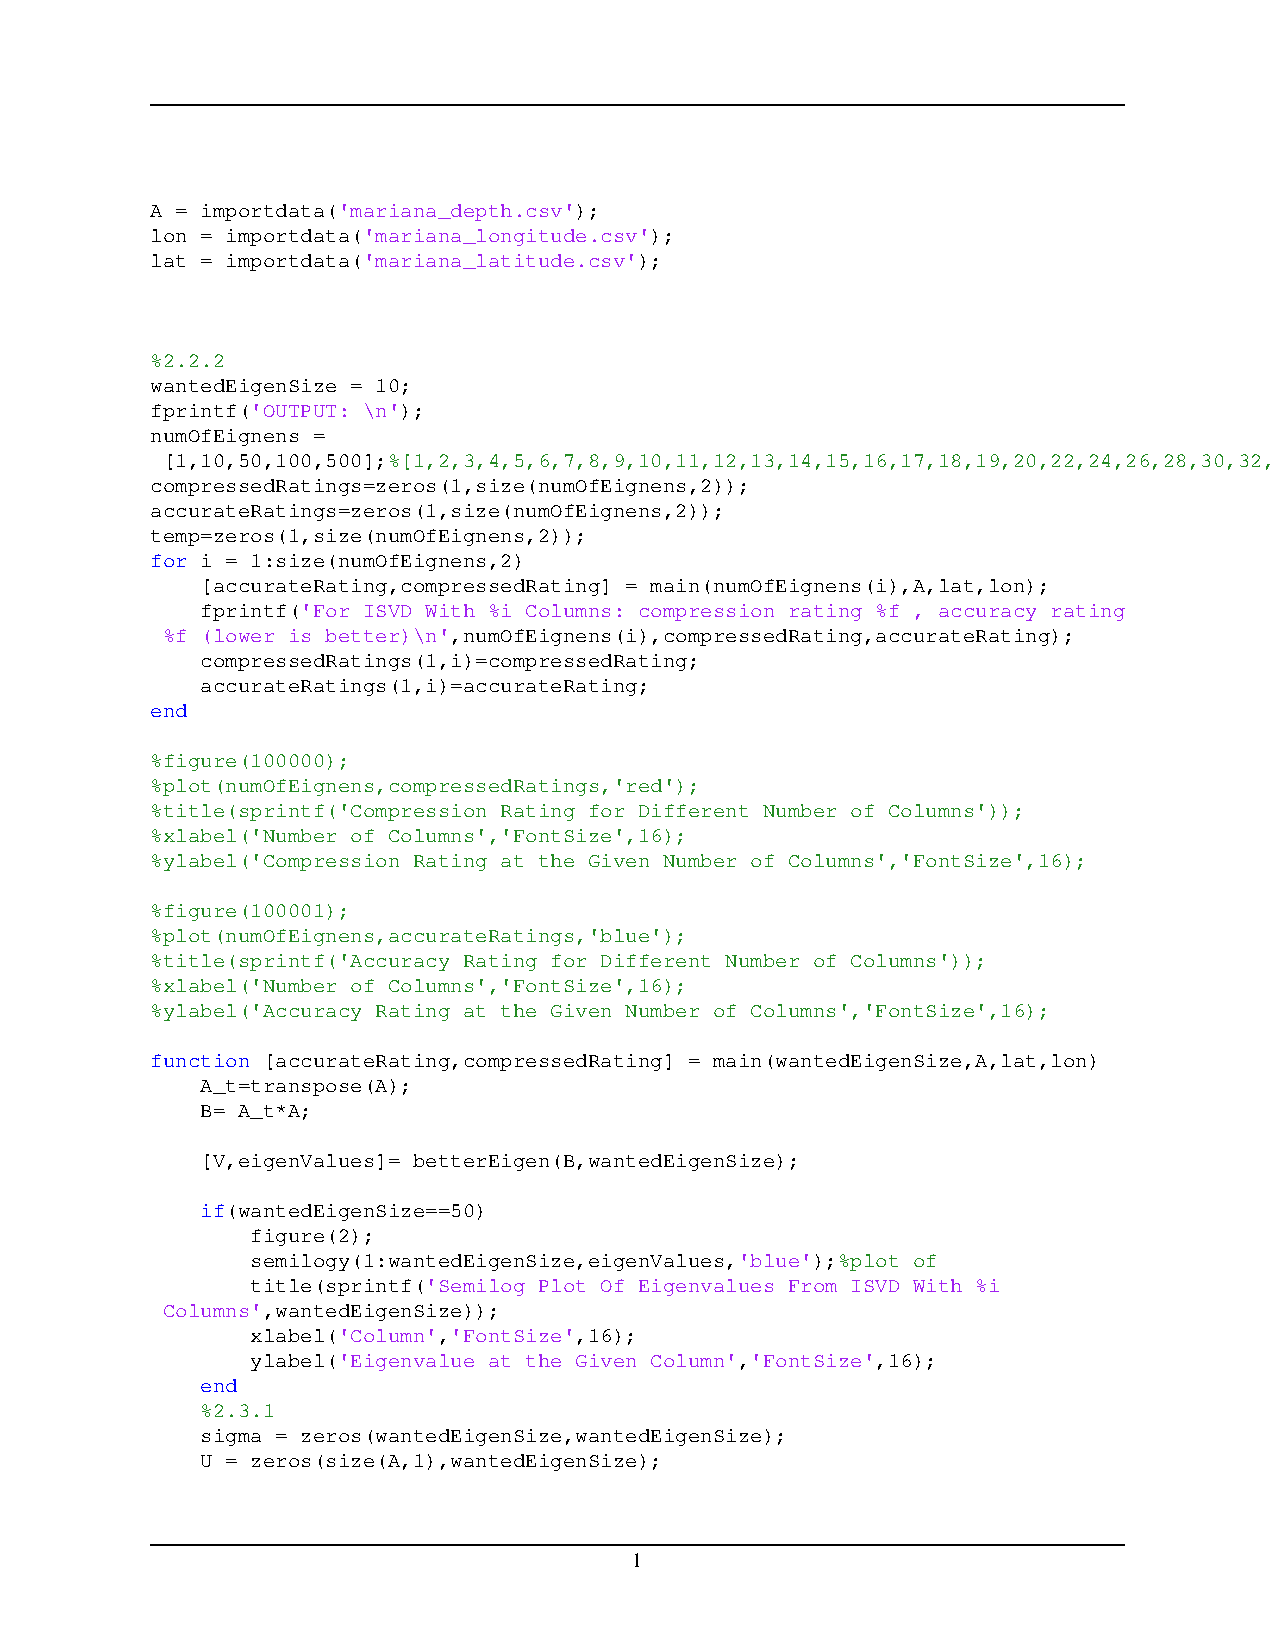
\includepdf[pages=-]{./referenceCode/Part222.pdf}







\end{document} % NOTHING AFTER THIS LINE IS PART OF THE DOCUMENT





